\documentclass[a4paper,12pt]{article}
\usepackage{settings} % Подгружает исправленный settings.sty
\usepackage{longtable}
\usepackage{graphicx}
\usepackage{float}
\usepackage{amsmath}

\begin{document}

% ==================== ТИТУЛЬНЫЙ ЛИСТ ====================
\thispagestyle{empty}

\begin{table}[h!]
\centering
\begin{tabular}{p{0.65\textwidth}r}
    \begin{tabular}{@{}l}
        \footnotesize{Университет ИТМО} \\
        \footnotesize{Физико-технический мегафакультет} \\
        \footnotesize{Физический факультет}
    \end{tabular} & 
    \raisebox{-0.5\height}{
\includegraphics[width=0.22\linewidth]{logo_ITMO.pdf}}
\end{tabular}
\end{table}

\vspace{0.5cm}

\begin{center}
\begin{tabular}{p{0.49\textwidth}p{0.49\textwidth}}
Группа \textbf{K3242} & К работе допущен \hrulefill \\
& \\
Студент \textbf{Шумилов А. К.} & Работа выполнена \hrulefill \\
& \\
Преподаватель \textbf{Курашова С. А.} & Отчет принят \hrulefill \\
\end{tabular}
\end{center}

\vspace{1.5cm}

\begin{center}
    \large{\textbf{Рабочий протокол и отчет по\\лабораторной работе № 3.13}} \\
    \vspace{0.8cm}
    \large{\textbf{«Магнитное поле Земли»}}
\end{center}

\newpage
\setcounter{page}{2}
\pagestyle{plain}

% ==================== ОСНОВНОЙ ТЕКСТ ====================

\section*{\hspace{30pt}1. Цель работы}
\hspace{15pt} Провести измерения направления суммарного магнитного поля, создаваемого Землей и системой катушек Гельмгольца. Определить горизонтальную составляющую магнитного поля Земли.

\section*{\hspace{30pt}2. Задачи, решаемые при выполнении работы}
\begin{enumerate}
    \setlength{\itemindent}{15pt}
    \item Провести юстировку компаса и ориентировать плоскость катушек под заданным углом к магнитному меридиану.
    \item Измерить зависимость силы тока в катушках от заданного угла отклонения магнитной стрелки.
    \item Рассчитать индукцию пробного магнитного поля катушек Гельмгольца $B_c$ для каждого значения тока.
    \item Построить график зависимости $B_c$ от геометрического фактора $\gamma$ и определить горизонтальную составляющую индукции магнитного поля Земли $B_h$ методом наименьших квадратов (МНК).
\end{enumerate}

\section*{\hspace{30pt}3. Объект исследования}
\hspace{15pt} Лабораторная установка, включающая последовательно соединенные кольца Гельмгольца, компас в центральной части, источник питания со встроенным амперметром и токоограничивающее сопротивление.

\section*{\hspace{30pt}4. Метод экспериментального исследования}
\hspace{15pt} Определение горизонтальной составляющей магнитного поля Земли $B_h$ базируется на суперпозиции земного магнитного поля и пробного поля $\vec{B}_c$, создаваемого катушками Гельмгольца. При наложении этих полей результирующий вектор отклоняет магнитную стрелку компаса. Измеряя угол отклонения $\alpha$ при различных значениях пробного поля, можно линейно связать эти величины и вычислить $B_h$.

\section*{\hspace{30pt}5. Рабочие формулы и исходные данные}
\hspace{15pt} Индукция однородного магнитного поля в центре катушек Гельмгольца рассчитывается по формуле:
\begin{equation}
    B_c = \mu_0 \left(\frac{4}{5}\right)^{\frac{3}{2}} \frac{I \cdot n}{R},
    \label{eq:bc_field}
\end{equation}
где $\mu_0 = 4\pi \cdot 10^{-7}$ Тл$\cdot$м/А — магнитная постоянная; $n = 100$ — число витков в каждой катушке; $R = 0.15$ м — средний радиус катушки; $I$ — средняя сила тока.

Для нахождения $B_h$ используется соотношение, полученное по теореме синусов для векторного треугольника полей:
\begin{equation}
    B_c = B_h \cdot \frac{\sin(\alpha_i)}{\sin(\varphi - \alpha_i)} = B_h \cdot \gamma_i,
    \label{eq:bh_calc}
\end{equation}
где $\varphi \approx 160^\circ$ — установочный угол между направлением поля катушек и геомагнитным меридианом; $\alpha_i$ — угол отклонения стрелки от начального положения. Величина $B_h$ определяется как угловой коэффициент линейной зависимости $B_c(\gamma_i)$.

\section*{\hspace{30pt}6. Измерительные приборы}
\begin{table}[H]
    \caption{Характеристики измерительных приборов стенда}
    \label{tab:devices}
    \centering
    \begin{tabular}{|c|c|c|c|c|}
        \hline
        № & Наименование & Тип & Диапазон & Погрешность \\ \hline
        1 & Амперметр & Цифровой & $0 \div 100$ мА & 1 мкА  \\ \hline
        2 & Компас & Механический & $0 \div 360^\circ$ & $1^\circ$  \\ \hline
    \end{tabular}
\end{table}

\section*{\hspace{30pt}7. Результаты прямых и косвенных измерений}
\hspace{15pt} В процессе выполнения эксперимента фиксировалось абсолютное положение стрелки компаса $\theta_i$. Угол отклонения стрелки рассчитывался как $\alpha_i = \varphi - \theta_i$, где $\varphi = 160^\circ$. Ниже представлены обработанные данные.

\begin{longtable}{|c|c|c|c|c|c|c|c|}
    \caption{Сводная таблица результатов измерений и вычислений} \label{tab:full_data} \\
    \hline
    $\theta_i$, $^\circ$ & $\alpha_i$, $^\circ$ & $I_1$, мА & $I_2$, мА & $I_3$, мА & $\langle I \rangle$, мА & $\gamma_i$ & $B_c$, мкТл \\ \hline
    \endfirsthead
    \multicolumn{8}{c}{{\bfseries \tablename\ \thetable{} -- Продолжение}} \\ \hline
    $\theta_i$, $^\circ$ & $\alpha_i$, $^\circ$ & $I_1$, мА & $I_2$, мА & $I_3$, мА & $\langle I \rangle$, мА & $\gamma_i$ & $B_c$, мкТл \\ \hline
    \endhead
    \hline \multicolumn{8}{|r|}{{Продолжение...}} \\ \hline
    \endfoot
    \hline
    \endlastfoot
    155 & 5 & 3.4 & 5.5 & 4.8 & 4.57 & 0.206 & 2.74 \\ \hline
    150 & 10 & 11.2 & 11.6 & 11.6 & 11.47 & 0.347 & 6.87 \\ \hline
    145 & 15 & 15.6 & 16.5 & 16.0 & 16.03 & 0.451 & 9.61 \\ \hline
    140 & 20 & 18.8 & 19.2 & 19.1 & 19.03 & 0.532 & 11.41 \\ \hline
    135 & 25 & 20.2 & 20.8 & 20.7 & 20.57 & 0.597 & 12.33 \\ \hline
    130 & 30 & 23.5 & 23.0 & 23.3 & 23.27 & 0.653 & 13.95 \\ \hline
    125 & 35 & 25.5 & 25.5 & 25.7 & 25.57 & 0.700 & 15.33 \\ \hline
    120 & 40 & 27.4 & 27.1 & 27.2 & 27.23 & 0.742 & 16.32 \\ \hline
    115 & 45 & 28.9 & 28.4 & 28.2 & 28.50 & 0.780 & 17.08 \\ \hline
    110 & 50 & 30.6 & 29.4 & 29.9 & 29.97 & 0.815 & 17.96 \\ \hline
    105 & 55 & 31.7 & 31.1 & 30.8 & 31.20 & 0.848 & 18.70 \\ \hline
    100 & 60 & 33.4 & 32.2 & 32.0 & 32.53 & 0.879 & 19.50 \\ \hline
    95 & 65 & 34.3 & 33.7 & 33.5 & 33.83 & 0.910 & 20.28 \\ \hline
    90 & 70 & 37.1 & 34.8 & 34.6 & 35.50 & 0.940 & 21.28 \\ \hline
    85 & 75 & 37.4 & 36.2 & 36.3 & 36.63 & 0.970 & 21.96 \\ \hline
    80 & 80 & 38.2 & 37.2 & 37.4 & 37.60 & 1.000 & 22.54 \\ \hline
    75 & 85 & 39.7 & 38.7 & 38.9 & 39.10 & 1.031 & 23.44 \\ \hline
    70 & 90 & 41.8 & 39.8 & 40.2 & 40.60 & 1.064 & 24.34 \\ \hline
    65 & 95 & 42.8 & 42.1 & 42.3 & 42.40 & 1.099 & 25.41 \\ \hline
    60 & 100 & 46.4 & 43.0 & 43.4 & 44.27 & 1.137 & 26.54 \\ \hline
    55 & 105 & 49.0 & 44.0 & 45.7 & 46.23 & 1.179 & 27.71 \\ \hline
    50 & 110 & 46.7 & 46.7 & 46.9 & 46.77 & 1.227 & 28.03 \\ \hline
    45 & 115 & 48.2 & 48.6 & 48.5 & 48.43 & 1.281 & 29.03 \\ \hline
    40 & 120 & 50.1 & 49.8 & 49.8 & 49.90 & 1.347 & 29.91 \\ \hline
    35 & 125 & 53.3 & 53.1 & 53.4 & 53.27 & 1.428 & 31.93 \\ \hline
    30 & 130 & 56.5 & 56.9 & 56.5 & 56.63 & 1.532 & 33.94 \\ \hline
    25 & 135 & 61.8 & 64.0 & 64.0 & 63.27 & 1.673 & 37.92 \\ \hline
\end{longtable}

\textit{Пример вычислений для первой строки:}
\begin{gather*}
    \langle I \rangle = \frac{3.4 + 5.5 + 4.8}{3} \approx 4.57 \text{ мА} \\
    B_c = 1.2566 \cdot 10^{-6} \cdot (0.8)^{1.5} \cdot \frac{4.57 \cdot 10^{-3} \cdot 100}{0.15} \approx 2.74 \cdot 10^{-6} \text{ Тл} = 2.74 \text{ мкТл} \\
    \gamma = \frac{\sin(5^\circ)}{\sin(160^\circ - 5^\circ)} = \frac{0.0871}{0.4226} \approx 0.206
\end{gather*}

\section*{\hspace{30pt}8. Обработка данных и вычисление погрешностей}
Определение горизонтальной составляющей $B_h$ сводится к нахождению углового коэффициента $b$ линейной зависимости $y = bx$, где $y_i = B_{c,i}$, $x_i = \gamma_i$. 

Согласно методу наименьших квадратов (МНК) для прямой, проходящей через начало координат:
\begin{gather*}
    b = B_h = \frac{\sum_{i=1}^{n} (\gamma_i \cdot B_{c,i})}{\sum_{i=1}^{n} \gamma_i^2} \approx 22.3 \text{ мкТл}
\end{gather*}

Для оценки случайной погрешности коэффициента $b$ найдем отклонения экспериментальных точек от аппроксимирующей прямой $d_i = B_{c,i} - b \cdot \gamma_i$ и вычислим среднее квадратичное отклонение $S_b$:
\begin{gather*}
    S_b = \sqrt{ \frac{1}{\sum \gamma_i^2} \cdot \frac{\sum d_i^2}{n - 1} } \approx 0.2 \text{ мкТл}
\end{gather*}
где $n = 27$ — количество измерений.

Абсолютная погрешность углового коэффициента с учетом коэффициента Стьюдента $t_{p, n-1} \approx 2$ (для доверительной вероятности $P=0.95$):
\begin{gather*}
    \Delta B_h = t \cdot S_b \approx 2 \cdot 0.2 = 0.4 \text{ мкТл}
\end{gather*}

\section*{\hspace{30pt}9. Графики результатов}
\begin{figure}[H]
    \centering
    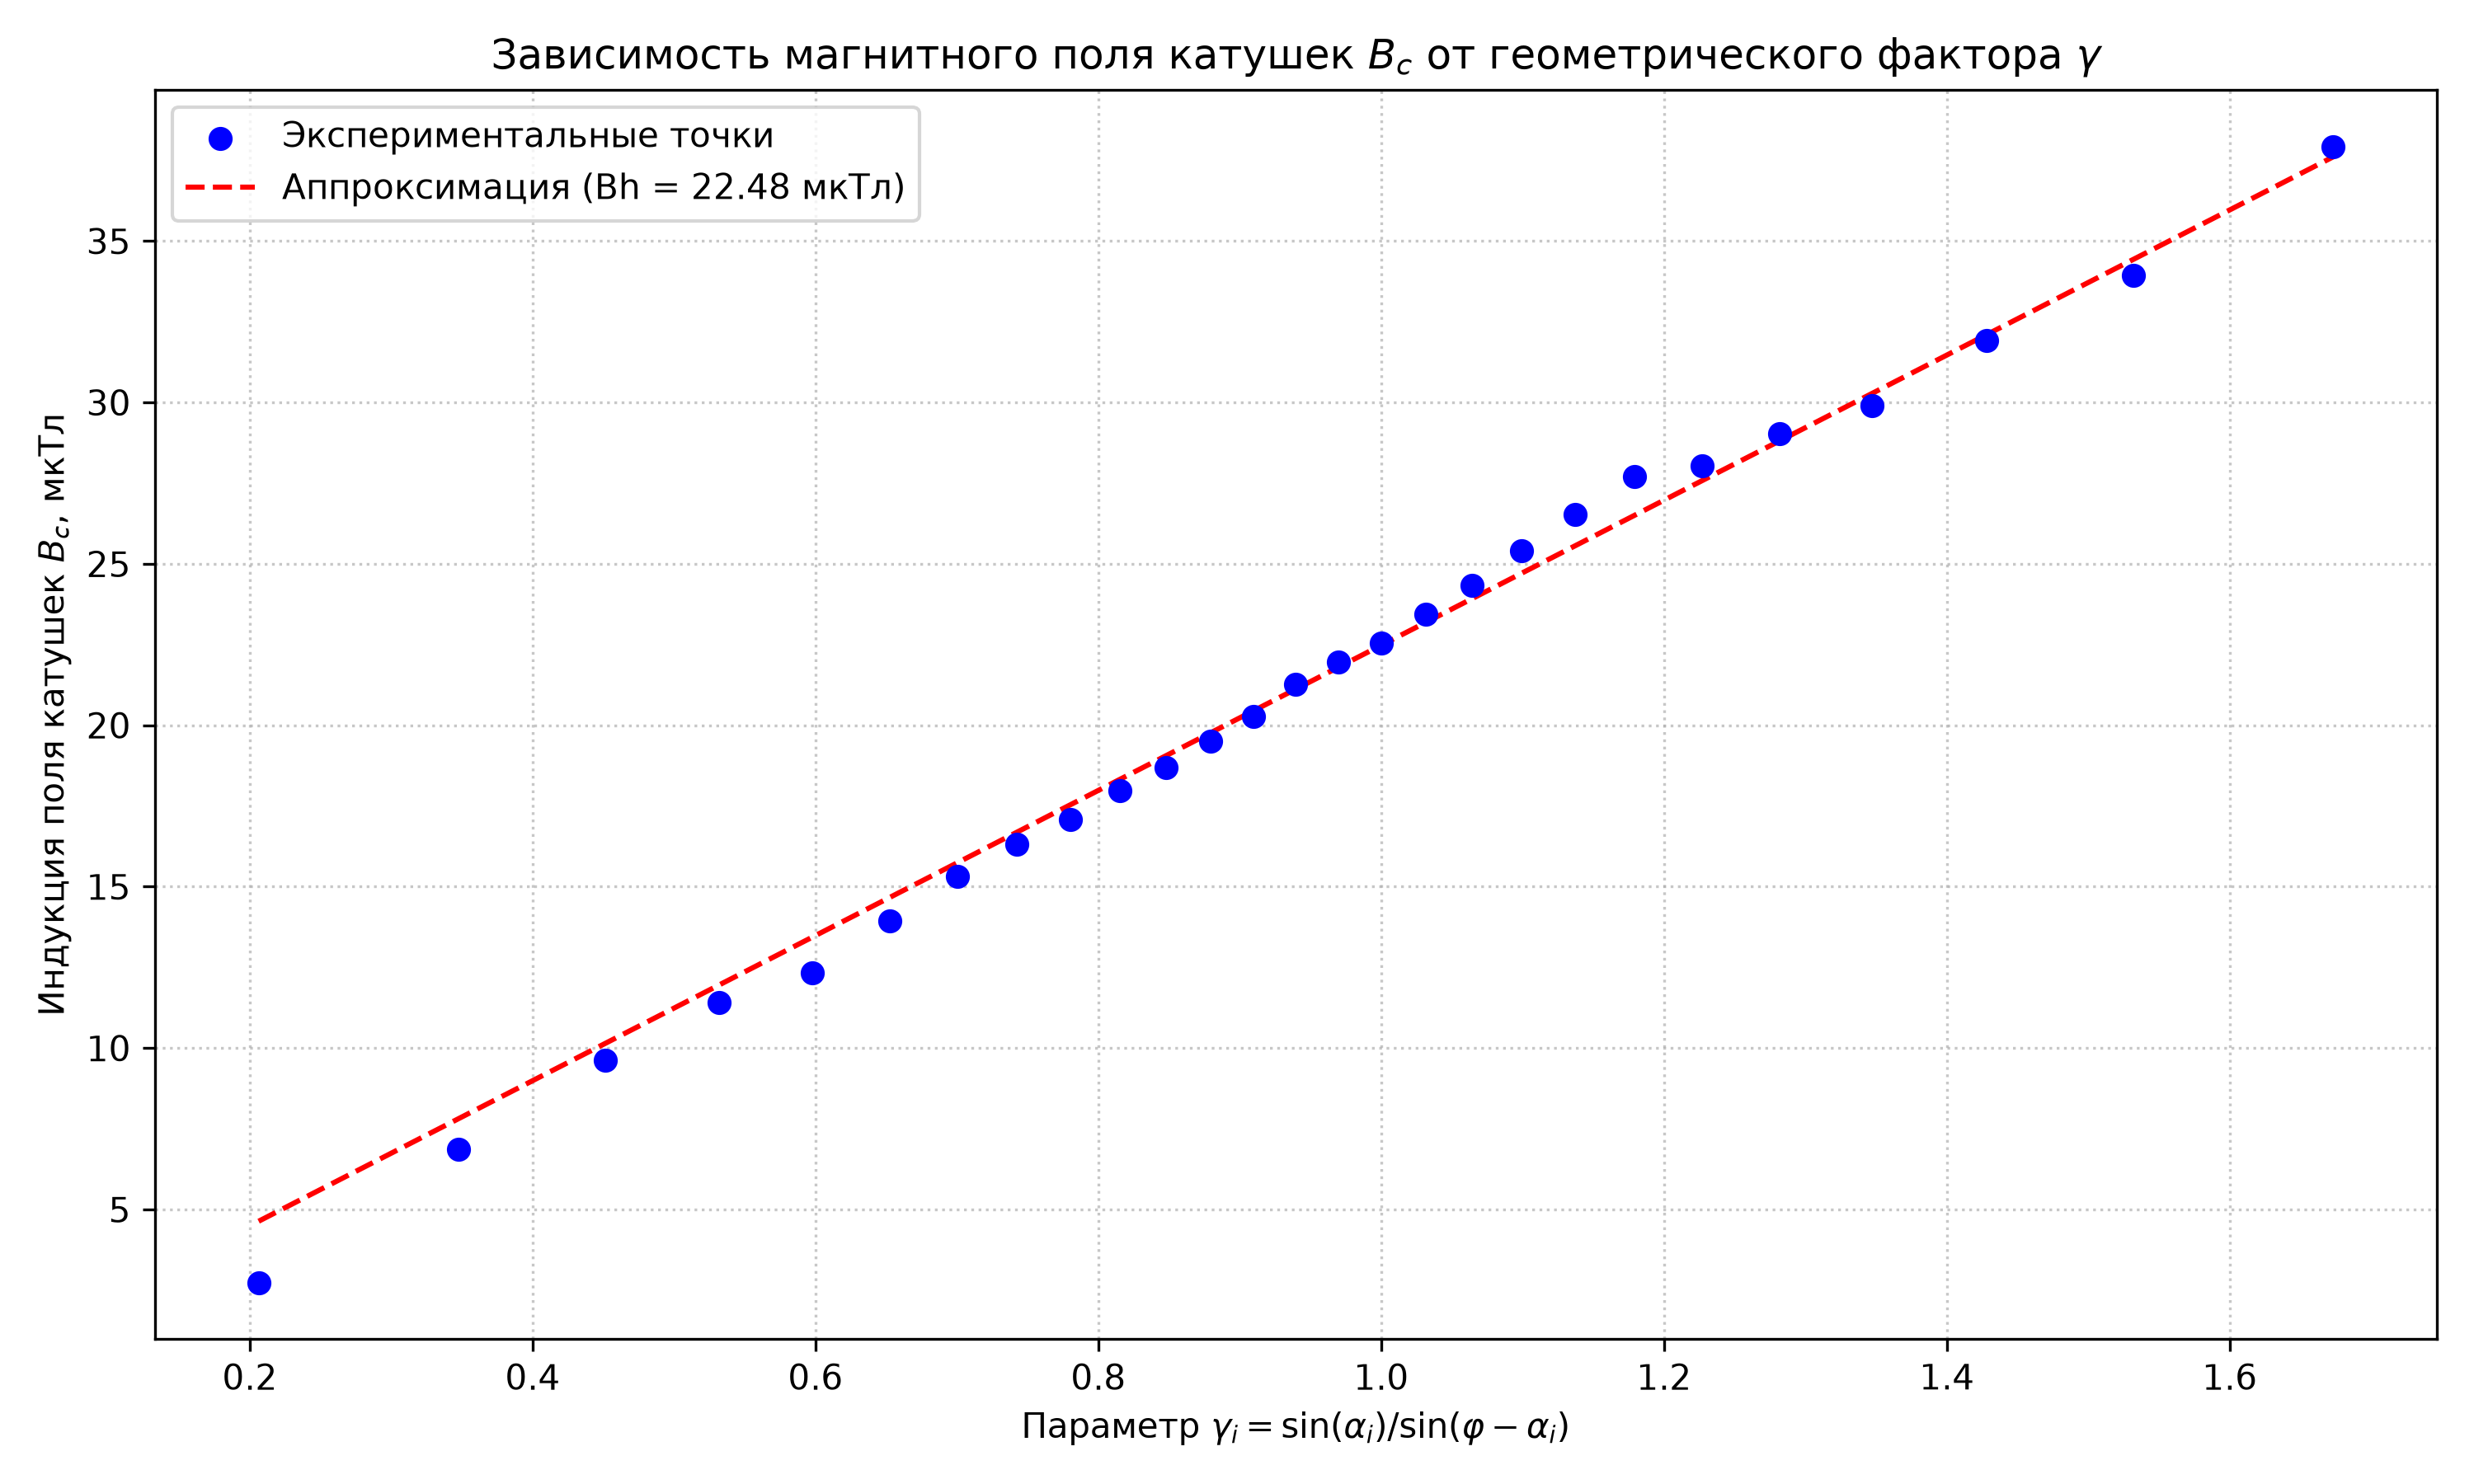
\includegraphics[width=0.9\textwidth]{fig1_magnetic_field.png}
    \caption{График зависимости поля катушек $B_c$ от геометрического параметра $\gamma_i$}
    \label{fig:regression}
\end{figure}

\section*{\hspace{30pt}10. Окончательные результаты}

\hspace{15pt} Табличное (справочное) значение горизонтальной составляющей магнитного поля Земли для Санкт-Петербурга:
\begin{equation*}
    B_{h,\text{табл}} \approx 15.46 \text{ мкТл} \text{ (соответствует } 12.3 \text{ А/м)}
\end{equation*}

Экспериментальное значение, полученное из наклона прямой:
\begin{equation*}
    B_h = (22.3 \pm 0.4) \text{ мкТл}
\end{equation*}

\section*{\hspace{30pt}11. Выводы и анализ результатов работы}

\hspace{15pt} В ходе лабораторной работы исследовано суммарное магнитное поле Земли и катушек Гельмгольца. Была построена линейная зависимость $B_c(\gamma_i)$, по угловому коэффициенту которой рассчитана горизонтальная составляющая геомагнитного поля.

\hspace{15pt} Полученное значение $B_h = 22.3 \pm 0.4$ мкТл отличается от табличного значения для Санкт-Петербурга (15.46 мкТл). Данное расхождение не покрывается случайной инструментальной погрешностью и объясняется сильным влиянием систематических факторов: наличием в аудитории посторонних ферромагнитных масс (металлические каркасы лабораторных столов, арматура здания) и побочных магнитных полей от электронного оборудования. Также свой вклад могла внести неидеальная изначальная ориентация установки по магнитному меридиану (погрешность установки угла $\varphi = 160^\circ$). Тем не менее, линейный характер зависимости $B_c$ от $\gamma_i$ (см. график) полностью подтверждает теоретическую модель суперпозиции магнитных полей, положенную в основу эксперимента.

\end{document}